\documentclass[a4paper, opensource]{./template/qyxf-book}
\usepackage{multicol}

\title{狭义相对论不得不说的那些事}
\subtitle{Key to Universal Physics}
\author{钱院学辅大物编写小组}
\typo{钱院学辅排版组}
\date{\today}
\version{v2.0}
\sourcepage{\url{https://github.com/qyxf/Tutorials/}}

\newcommand{\di}[1]{\mathrm{d}#1}
\newcommand{\p}[2]{\frac{\partial #1}{\partial #2}}
\newcommand{\pp}[2]{\frac{\partial ^2 #1}{\partial #2 ^2}}
\newcommand{\dy}[2]{\frac{\di{#1}}{\di{#2}}}
\newcommand{\ddy}[2]{\frac{\mathrm{d} ^2 #1}{\mathrm{d} #2 ^2}}

\begin{document}
\maketitle
\begin{section}{洛伦兹变换、尺缩公式和钟缓公式}
初学者经常会搞不清楚这三个公式的适用条件,事实上这三个公式并不是同一“层次”的公式。洛伦兹变换描述的是在不同参考系中看同一事件的方法,而尺缩钟缓是洛伦兹变换的导出关系。

\begin{subsection}{钟缓}
对于$S'$系中的两个事件:他们之间仅有时间间隔,没有空间间隔
\begin{equation*}
A(x',y',z',t_1') \hspace{4em} B(x',y',z',t_2')
\end{equation*}
在$S$系中有
\begin{equation*}
A(\frac{x'+vt_1'}{\sqrt{1-\beta^2}},\gamma',z',\frac{t_1'+\frac{v}{c^2}x'}{\sqrt{1-\beta^2}}) \hspace{4em} 
B(\frac{x'+vt_2'}{\sqrt{1-\beta^2}},\gamma',z',\frac{t_2'+\frac{v}{c^2}x'}{\sqrt{1-\beta^2}})
\end{equation*}
$S$系中看到的两事件时间间隔
\begin{equation*}
\Delta t = t_B - t_A = \frac{t_2'-t_1'}{\sqrt{1-\beta^2}} = \frac{\Delta t'}{\sqrt{1-\beta^2}} \hspace{4em}
\end{equation*}
即为钟缓公式.
\end{subsection}

\begin{subsection}{尺缩}
对于$S'$系中的两个事件:它们之间仅有空间间隔
\begin{equation*}
A(x_1',y',z',t') \hspace{4em} B(x_2',y',z',t')
\end{equation*}
$S$系中
\begin{equation*}
A(\frac{x_1'+vt'}{\sqrt{1-\beta^2}},y',z',\frac{t'+\frac{v}{c^2}x_1'}{\sqrt{1-\beta^2}}) \hspace{4em}
B(\frac{x_2'+vt'}{\sqrt{1-\beta^2}},y',z',\frac{t'+\frac{v}{c^2}x_2'}{\sqrt{1-\beta^2}})
\end{equation*}
$S$系中两事件空间间隔
\begin{equation*}
\Delta x = x_B - x_A = \frac{x_2'-x_1'}{\sqrt{1-\beta^2}} = \frac{\Delta x'}{\sqrt{1-\beta^2}}
\end{equation*}
故尺缩公式为
\begin{equation*}
l'=\sqrt{1-\beta^2}
\end{equation*}
\end{subsection}

\begin{subsection}{注意事项}
这里有一个误区(坑),很多人,尤其是初学者,喜欢对于$S'$系中的两个事件的空间间隔应用尺缩公式。但是,其实这是不正确的,尺缩仅仅是对于$S'$系或$S$系中实实在在的尺子才可以使用的。准确来说,尺缩公式是这样推导出来的:

在$S$系中有两个事件:$A$:看尺子前端$(x_1,y_1,z_1,t_1)$

\hspace{10em} $B$:看尺子后端$(x_2,y_2,z_2,t_2)$ \hspace{4em} $(y_1=y_2,z_1=z_2)$

在$S'$系中
\begin{equation*}
x_1'=\frac{x_1-vt_1}{\sqrt{1-\beta^2}} \hspace{4em} x_2'=\frac{x_2-vt_2}{\sqrt{1-\beta^2}}
\end{equation*}
$S$系中空间间隔
\begin{equation*}
x_1'-x_2'=\frac{(x_1-x_2)-v(t_1-t_2)}{\sqrt{1-\beta^2}}
\end{equation*}
但是测量尺长时,$S$系中尺子是动的,$S'$系中尺子是不动的,因此为了保证$S$系中测得尺长的准确,应当同时看前后两端
\begin{equation*}
t_1=t_2
\end{equation*}
则
\begin{equation*}
x_1'-x_2'=\frac{x_1-x_2}{\sqrt{1-\beta^2}} \hspace{2em} \Rightarrow \hspace{2em}
x_1-x_2=(x_1'-x_2')\sqrt{1-\beta^2}=L\sqrt{1-\beta^2}
\end{equation*}
因此:尺缩公式不是长度变换(或距离变换),对于$S'$系中同时发生的事件,在$S$系中看要用洛伦兹变换,洛伦兹变换才是求解相对论问题的正确打开方式.
\end{subsection}

\begin{subsection}{小结}
$S'$系中同地不同时$ \rightarrow S$系 \hspace{2em} 用钟缓.

$S'$系中长度固定不变$ \rightarrow S$系 \hspace{1em} 用尺缩.

其他$S \rightarrow S'$和$S' \rightarrow S$ \hspace{4em}对每个事件用洛伦兹变换,然后作差.
\end{subsection}

\exercise{例题:作业第一题}
飞船以$u=0.6c$飞离地球.假设头部向尾部发出一个光讯号.飞船上经$\Delta t'=1\mu s$后尾部接受器接收到该信号,求地面上观测者测得光讯号到达船尾的时间$\Delta t$.

\solve
\begin{multicols}{2}
解:以飞船参考系为$S'$系,地面系为$S$系.\\
在飞船系中,事件$A$:发出光,事件$B$,接受光.\\
在$S$系中,对$A$:$(\beta=\frac{u}{c})$
\begin{equation*}
x_A=\frac{x_A'+ut_A'}{\sqrt{1-\beta^2}} \hspace{4em} 
t_A=\frac{t_A'+\frac{u}{c^2}x_A'}{\sqrt{1-\beta^2}} \hspace{4em}
\end{equation*}
对$B$:
\begin{equation*}
x_B=\frac{x_B'+ut_B'}{\sqrt{1-\beta^2}} \hspace{4em}
t_B=\frac{t_B'+\frac{u}{c^2}x_B'}{\sqrt{1-\beta^2}}
\end{equation*}

\hspace{4em}
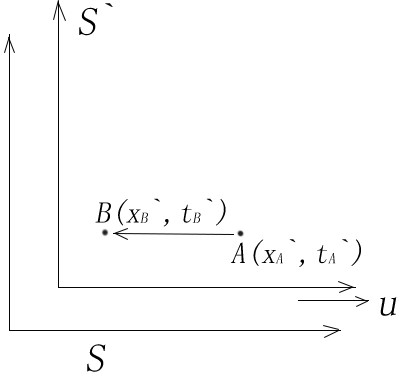
\includegraphics[scale=0.5]{Chp5_addin_illus1.jpg}
\end{multicols}

$S$系中的时间差:
\begin{equation*}
\Delta t = t_B - t_A = \frac{(t_B'-t_A')+\frac{u}{c^2}x_B'}{\sqrt{1-\beta^2}}
\end{equation*}
在$S'$系中,光沿$x'$负方向:$x_B'-x_A'=-c(t_B'-t_A')$

即
\begin{equation*}
\Delta t=\frac{1-\beta}{\sqrt{1-\beta^2}}(t_B'-t_A')=\sqrt{\frac{1-\beta}{1+\beta}}\Delta t
=0.5\mu s
\end{equation*}

分析:

对洛伦兹变换的理解:观察者站在\underline{不同参考系}中观测事件引发的事件的\underline{空间坐标和时间坐标}的变化.

在同一参考系中,某些经典力学的结论仍然成立.\\

\exercise{作业18题第一空}
地面参考系中工作人员发射脉冲信号时间间隔为$3s$,地面上工作人员看两信号被接受的时间间隔\underline{\hspace{2em}}$s$.

\solve
因为不涉及参考系的变换,两个都是在地面系中观察,这就是一个\underline{\underline{普通}}的追及问题.

\
$A$信号被接收时:\qquad
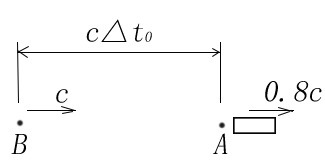
\includegraphics[scale=0.5]{Chp5_addin_illus2.jpg}

因此时间差为
\begin{equation*}
\Delta t=\frac{c\Delta t_0}{c-0.8c}=5\Delta t_0=15s
\end{equation*}

是的,这一小问没有使用相对论.


\end{section}

\begin{section}{速度变换的一点小问题}
\begin{multicols}{2}
采用微分法推导速度变换\hspace{2em}$\beta=\frac{u}{c}$
\begin{align*}
\begin{cases}
\di x'=\frac{\di x-v\di t}{\sqrt{1-\beta^2}}\\[6pt]
\di y'=\di y\\[6pt]
\di z'=\di z\\[6pt]
\di t'=\frac{\di t-\frac{v\di x}{c^2}}{\sqrt{1-\beta^2}}
\end{cases}
\end{align*}
算出速度变换
\begin{align*}
\begin{cases}
u_x'=\frac{\di x'}{\di t'}=\frac{u_x-v}{1-\frac{vu_x}{c^2}}\\[6pt]
u_y'=\frac{\di y'}{\di t'}=\frac{u_y\sqrt{1-\beta^2}}{1-\frac{vu_x}{c^2}}\\[6pt]
u_z'=\frac{\di z'}{\di t'}=\frac{u_z\sqrt{1-\beta^2}}{1-\frac{vu_x}{c^2}}
\end{cases}
\end{align*}

\hspace{4em}
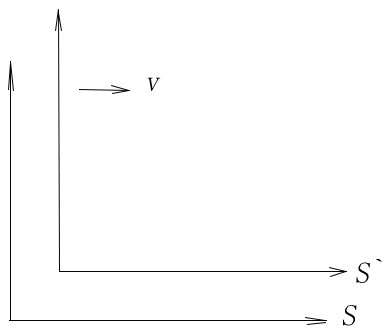
\includegraphics[scale=0.6]{Chp5_addin_illus3.jpg}
\end{multicols}
其中,$u_x'\Rightarrow\hspace{2em} S\rightarrow S'$系,相对速度小于绝对速度,因此都为减(可以与伽利略速度变换比较$u_x'=u_x-v$).
$u_y'$和$u_z'$在伽利略变换中实际上不变.

逆变换
\begin{align*}
\begin{cases}
u_x=\frac{u_x'+v}{1+\frac{vu_x}{c^2}}\\[6pt]
u_y=\frac{u_y'\sqrt{1-\beta^2}}{1+\frac{vu_y'}{c^2}}\\[6pt]
u_z=\frac{u_z'\sqrt{1-\beta^2}}{1+\frac{vu_z'}{c^2}}
\end{cases}
\end{align*}

对比伽利略变换
\begin{align*}
\begin{cases}
u_x=u_x'+v\\
u_y=u_y'\\
u_z=u_z'
\end{cases}
\end{align*}
\end{section}

\begin{section}{关于能量}
与经典不同之处在于,引入了总能量$E=mc^2$(爱因斯坦指出,$m$比$\frac{m_0}{\sqrt{1-\beta^2}}$更恰当)

静能\qquad$E_0=m_0c^2$

总能\qquad$E=mc^2$

动能\qquad$E_k=E-E_0=mc^2-m_0c^2$

由几个公式可以推导出$E^2=p^2c^2+m_0^2c^4$

$\bigcirc$因此:在相对论的世界中,只有动能是不容易确定的,它应由总能量与静能相减得到.

总能量和静能都可以由静质量和动质量得到.

在这一部分的计算中,更多是一些原子物理方面的情境,比如$\Lambda^0$超子衰变.

在原子物理中使用的单位制是:质量$MeV/c^2\hspace{2em}$能量$MeV\hspace{2em}$动量$MeV/c$

因此较为方便计算,没有必要为光速$c$烦恼.

$\bigcirc$解题方面:

(1)总能量之和不变(即能量守恒).

(2)碰撞、衰变、分裂过程中动量守恒.

(3)直接的结论就是粒子的静质量之和不守恒$\rightarrow$质量亏损.
\end{section}

\begin{section}{拓展内容}
\begin{subsection}{关于历史问题的一点叙述}
麦克斯韦电磁理论与相对性原理的冲突:

在牛顿时代,人们发现了这样一条定律,“物理定律在所有惯性系中都有相同的数学形式”。事实上,牛顿的经典力学中的每一个定律都遵循这样的一条规律。这样的一条定律是物理学中对称性的体现。经过长期的理论研究发现,这条定律约束着其他的规律。它是一条“管定律的定律”。好景不长,麦克斯韦建立了它的电磁理论后,发现了这样的矛盾
\begin{equation*}
\mbox{水火不容?}
\begin{array}{c}
\nearrow\\\searrow
\end{array}
\begin{array}{l}
\mbox{(1)麦克斯韦方程:光速为$c$}\\\mbox{(2)相对性原理:协变性}
\end{array}
\Bigg\}
\Rightarrow
\mbox{光速对各系为$c$}
\stackrel{?}{\iff}
\mbox{与伽利略变换矛盾}
\end{equation*}
仔细思考:原牛顿力学中的相对性原理是由伽利略变换导出的,但是原相对性原理应该是可以和麦氏方程相容的。真正水火不容的氏麦氏方程和伽利略变换。只有默认相对性原理是由伽利略变换得到的才会遇到这样的矛盾。爱因斯坦的功劳在于他敏锐地发现伽利略变换的不完善性,并使用数年前洛伦兹得到的变换式去修正伽利略变换,进而使麦氏方程与修正后的相对性原理相容。我们可以发现,狭相的两条假设分别对应着相对性原理和麦克斯韦方程组,而整个相对论体系是适用于宏观高速的一切定律的。
\end{subsection}

\begin{subsection}{关于洛伦兹变换和尺缩、钟缓公式}
1.理解“事件”:相对论中需要抓住的一个要点即是“事件”

对于事件$A(x,y,z,t)$,其时空坐标在不同参考系是不同的,我们可以用洛伦兹变换将事件的$S$系中的坐标$(x,y,z,t)$换到$S'$系中,得到$S$系坐标$(x',y',z',t')$

2.洛伦兹变换的实质
\begin{multicols}{2}
\hspace{4em}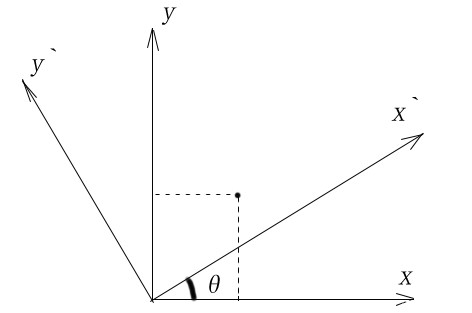
\includegraphics[scale=0.5]{Chp5_addin_illus4.jpg}

空间中坐标$(x,y)$,在$S$系中坐标为
\begin{equation*}
\begin{bmatrix}
x'\\y'
\end{bmatrix}
=
\begin{bmatrix}
\cos{\theta} & \sin{\theta}\\-\sin{\theta} & \cos{\theta}
\end{bmatrix}
\begin{bmatrix}
x\\y
\end{bmatrix}
\end{equation*}

\end{multicols}
洛伦兹变换
\begin{equation*}
\begin{bmatrix}
ct\\x\\y\\z
\end{bmatrix}
=
\begin{bmatrix}
\frac{1}{\sqrt{1-\beta^2}}&\frac{\beta}{\sqrt{1-\beta^2}}\\
\frac{\beta}{\sqrt{1-\beta^2}}&\frac{1}{\sqrt{1-\beta^2}}\\
&&1\\
&&&1
\end{bmatrix}
\begin{bmatrix}
ct'\\x'\\y'\\z'
\end{bmatrix}
\end{equation*}
洛伦兹变换实际上是四维时空(闵氏空间)中的旋转变换.
\end{subsection}

\begin{subsection}{例题}
\begin{multicols}{2}
\exercise{: 例1}$A$ , $B$ 为宇宙中的两艘飞船,$A$以速度$v=\beta c$沿$x$轴正方向飞行,$B$ 以速度 $v=\beta c$ 沿 $x$轴负方向飞行。两者在$S$系中观察,$y$ 方向上由 $y_B-y_A=d$,当在$S$系中,$A$、$B$之间距离最短时,由$A$向$B$发出一束光信号,问:

\hspace{3em}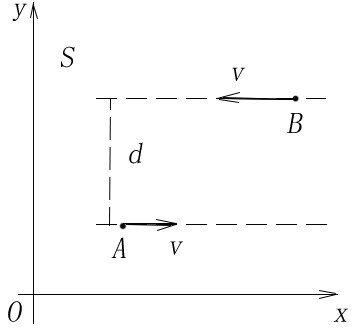
\includegraphics[scale=0.3]{Chp5_addin_illus5.jpg}
\end{multicols}
1.以$A$为参考系,$A$应该按什么方向发射光信号,使$B$接收到?

\analysis 如果按$S$系算,那就先勾股定理,然后还要换成$A$系,很明显,这有些麻烦.

不如直接以$A$为参照系,此时$B$的相对速度
\begin{equation*}
v'=\frac{v-(-v)}{1-\frac{v\cdot(-v)}{c^2}}=\frac{2\beta}{1+\beta^2}c
\end{equation*}

当我们站在飞船上,$B$是这样运动的:

\hspace{17em}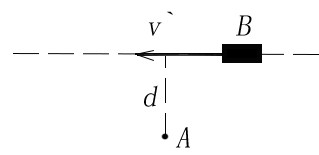
\includegraphics[scale=0.6]{Chp5_addin_illus6.jpg}

距离最短时,$A$发出光,但是肯定不是指向$B$,情况是这样:

\hspace{17em}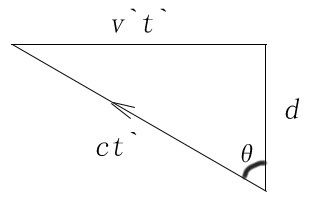
\includegraphics[scale=0.6]{Chp5_addin_illus7.jpg}

$t'$为光信号在$A$系中传播的时间,由勾股定理
\begin{align*}
(v't')^2+d^2&=(ct')^2\\\tan{\theta}&=\frac{v't'}{d}
\end{align*}

最终解得光信号与$x$轴正向夹角$\varphi=\frac{1}{2}\pi+\theta=\frac{1}{2}\pi+\arctan{\frac{2\beta}{1-\beta^2}}$

有没有更简单的?

仔细看可以发现$\sin{\theta}=\frac{v't'}{ct'}=\frac{2\beta}{1+\beta^2}$

夹角$\varphi$可以表示为$\varphi=\frac{1}{2}\pi+\arcsin{\frac{2\beta}{1+\beta^2}}$

(好吧,第一种解法只是我硬写的计算方式,大家忽略吧......)

\exercise{:例题2}$B$接收到信号时,$B$中宇航员认为自己与$A$相距多少?$B$宇航员的眼中,$A$是怎样的?

(1)首先距离最短时\hspace{2em}(2)$A$向$B$发了束光\hspace{2em}(3)光到了$B$\hspace{2em}(4)没了......

\hspace{3em}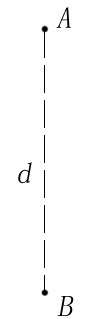
\includegraphics[scale=0.5]{Chp5_addin_illus8.jpg}
\hspace{7em}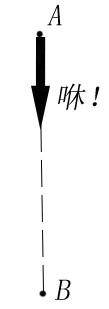
\includegraphics[scale=0.5]{Chp5_addin_illus9.jpg}
\hspace{5em}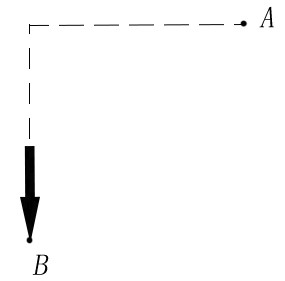
\includegraphics[scale=0.5]{Chp5_addin_illus10.jpg}

那时间呢?

\solve
$B$系:$t''=\frac{d}{c}$(光是正冲着$B$发出去的)

而$A$的速度不难求\hspace{2em}$v_A'=\frac{2\beta}{1+\beta^2}c$为$A$相对$B$的速度.

由此$A$与$B$相距同样可以利用勾股定理
\begin{equation*}
L_(AB)=\sqrt{d^2+(v_A''t'')^2}=\frac{\sqrt{(1+\beta^2)^2+4\beta^2}}{1+\beta^2}d
\end{equation*}

我们再看第1问,以$A$为参考系,从发光到$B$接收光时间
\begin{equation*}
t'=\frac{d}{c}=\frac{1+\beta^2}{1-\beta^2}
\end{equation*}

这与$t''$是不一样的,大家不要想当然地代错时间.

\exercise{: 例3}关于能量与质量的理解:

太空火箭的初始质量$M_0$,从静止起飞,向后喷出的气体相对火箭速度为常数$u$,任意时刻设火箭的速度为$v$,静止质量为$m_0$,试求$\frac{m_0}{M_0}$与$v$的关系.

\solve 设在地球参考系中,时刻$t$火箭的质量为$m$(是质量,不是静止质量).
\begin{equation*}
m=\frac{m_0}{\sqrt{1-\beta^2}}\hspace{4em}\beta=\frac{v}{c}
\end{equation*}

设火箭在$t$时刻喷出$\di m$气体,这部分气体与火箭系统动量守恒,但我们先要换到地球参考系,系中的
\begin{equation*}
v_{\mbox{气}}=\frac{u-v}{1-\frac{uv}{c^2}}
\end{equation*}
方向向下.

列动量守恒:$mv=(m-|\di m|)(v+\di v)+v_{\mbox{气}}|\di m|$

而火箭质量是一直减的($\di m<0$),因而有
\begin{equation}
|\di m|=-\di m=-\di(\frac{m_0}{\sqrt{1-\beta^2}})
\end{equation}
带入化简得
\begin{equation}
\frac{m_0}{\sqrt{1-\beta^2}}\di v+(v+v_{\mbox{气}})\di(\frac{m_0}{\sqrt{1-\beta^2}})=0
\end{equation}

这是忽略高阶小量后的表达式

(1)(2)式代入得
\begin{equation*}
\frac{m_0}{\sqrt{1-\beta^2}}\di v+\frac{u(1-\beta^2)}{1-\frac{u}{c}\beta^2}[\frac{\di m_0}{\sqrt{1-\beta^2}}
+m_0\frac{v}{c^2}\frac{\di v}{(1-\beta^2)^{\frac{3}{2}}}]=0
\end{equation*}

化简后得$m_0\di v=u(\beta^2-1)\di m_0$

之后是一系列的积分得
\begin{equation*}
\ln m_0=\frac{c}{2u}\ln \frac{1-\beta}{1+\beta}+C
\end{equation*}

$t=0$时$\beta=0\hspace{1em}m_0=M_0$,故$C=\ln M_0$

代入式子得
\begin{equation*}
\frac{m_0}{M_0}=(\frac{1-\beta}{1+\beta})^{\frac{c}{2u}}
\end{equation*}

如果是考试,应该不会出像这样数学成分比较多的题,主要是注意下动量守恒的式子,有些人可能会这样写
\begin{equation*}
\frac{M_0}{\sqrt{1-\beta^2}}v=(\frac{m_0}{\sqrt{1-\beta^2}}+\frac{\di m_0}{\sqrt{1-\beta^2}})(v+\di v)
-v_{\mbox{气}}(\frac{-\di m_0}{\sqrt{1-\beta^2}})
\end{equation*}

肯定不对.建议大家列动量守恒式时先用动质量$m$,再谨慎地换为静质量$m_0$.
\end{subsection}
\end{section}

\begin{section}{写在后面}
以上只是做题时,自己的一些想法......

如果你有一套自己的做题体系,那还是不要轻易改变,毕竟相对论的题,在$S$系看能做出来,在$S'$系看也能做,我写的只是我认为的“建议”。

如果你是高数大佬,或者C++大神,欢迎向钱院学辅投稿,写点小助手啥的。

祝大家相对论学习顺利!
\end{section}
\end{document}